\documentclass{ximera}
\graphicspath{
{./}
{volumes/}
{arclengths/}
{centroids/}
{techniques/}
{applications/}
{series/}
{powerseries/}
{odes/}
{lessons/}
}
\usepackage{booktabs}

\newcommand{\bigmath}[1]{$\displaystyle #1$}
\newcommand{\choicebreak}{}
\newenvironment{type}{}{}
\newenvironment{notes}{}{}
\newenvironment{keywords}{}{}
\newcommand{\offline}{}
\newenvironment{comments}{\begin{feedback}}{\end{feedback}}
\newenvironment{multiplechoice}{\begin{multipleChoice}}{\end{multipleChoice}}
\title{Exercises: Shell Method}
\author{Philip T. Gressman}

\begin{document}
\begin{abstract}
Exercises for using the shell method.
\end{abstract}
\maketitle

\begin{exercise}
The region defined by the inequalities $\sqrt{1-x^2} \leq y \leq 1$ for $0 \leq y \leq 1$ is revolved around the $y$-axis. Compute the volume of the resulting solid using the shell method.
\begin{center}
\begin{image}
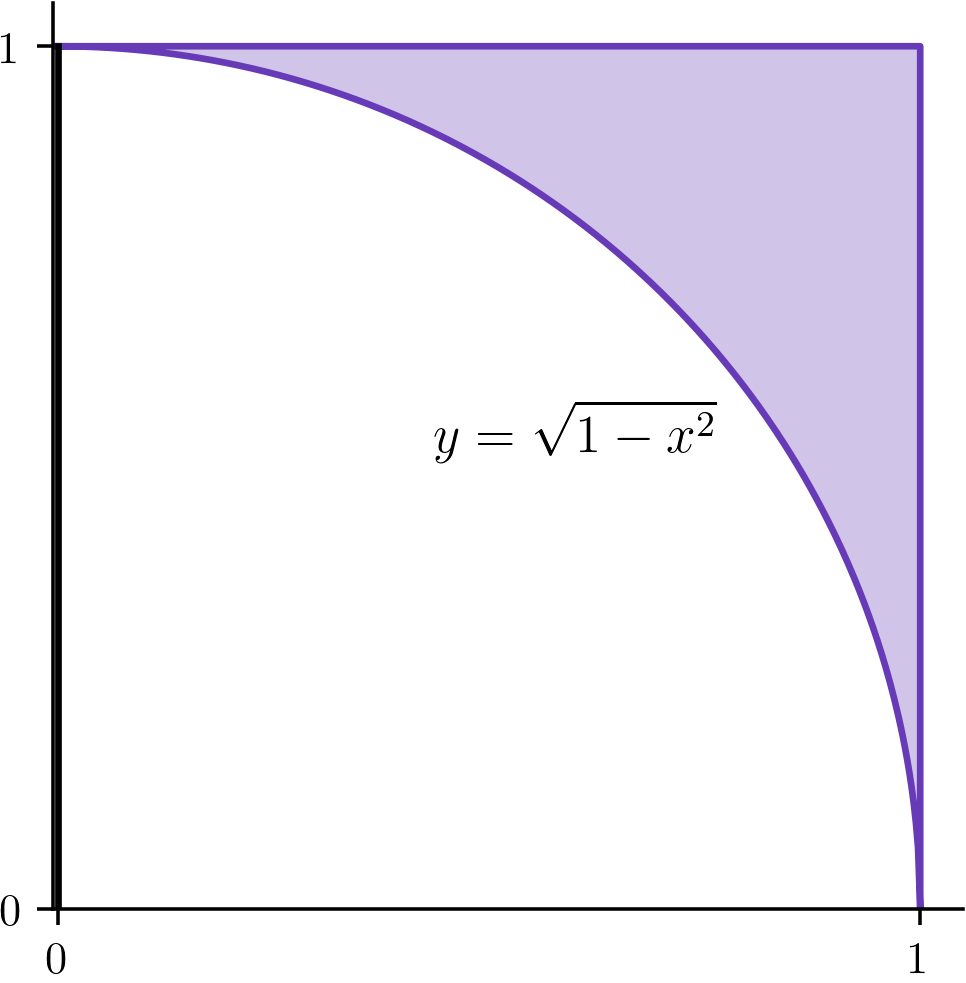
\includegraphics{shell/shell03.png}
\end{image}
\end{center}
\begin{itemize}
\item When the slicing variable is $x$, the radius of a shell is the \wordChoice{\choice[correct]{horizontal}\choice{vertical}} distance from an $x$-slice to the axis of rotation. Thus
\[ r(x) = \answer{x} - \answer{0}. \]
\item The height of an $x$-slice is equal to
\[ h(x) = \answer{1 - \sqrt{1 - x^2}}. \]
\item The volume is equal to the integral of $2 \pi r h$, so 
\[ V = \int_{\answer{0}}^{\answer{1}} \answer{2 \pi x ( 1 - \sqrt{1-x^2}) } dx = \answer{\frac{\pi}{3}}. \]
(Note: to compute the integral, split it into two parts and make the substitution $u = 1-x^2$ for one of them.)
\end{itemize}
\end{exercise}

\begin{exercise}
The region in the plane bounded above by the graph $y = \sqrt{1+x^2}$, below by $y = -1 + x + \sqrt{1+x^2}$, and on the left by $x = 0$ is revolved around the axis $x = 1$. Compute the volume of the resulting solid using the shell method.
\begin{center}
\begin{image}
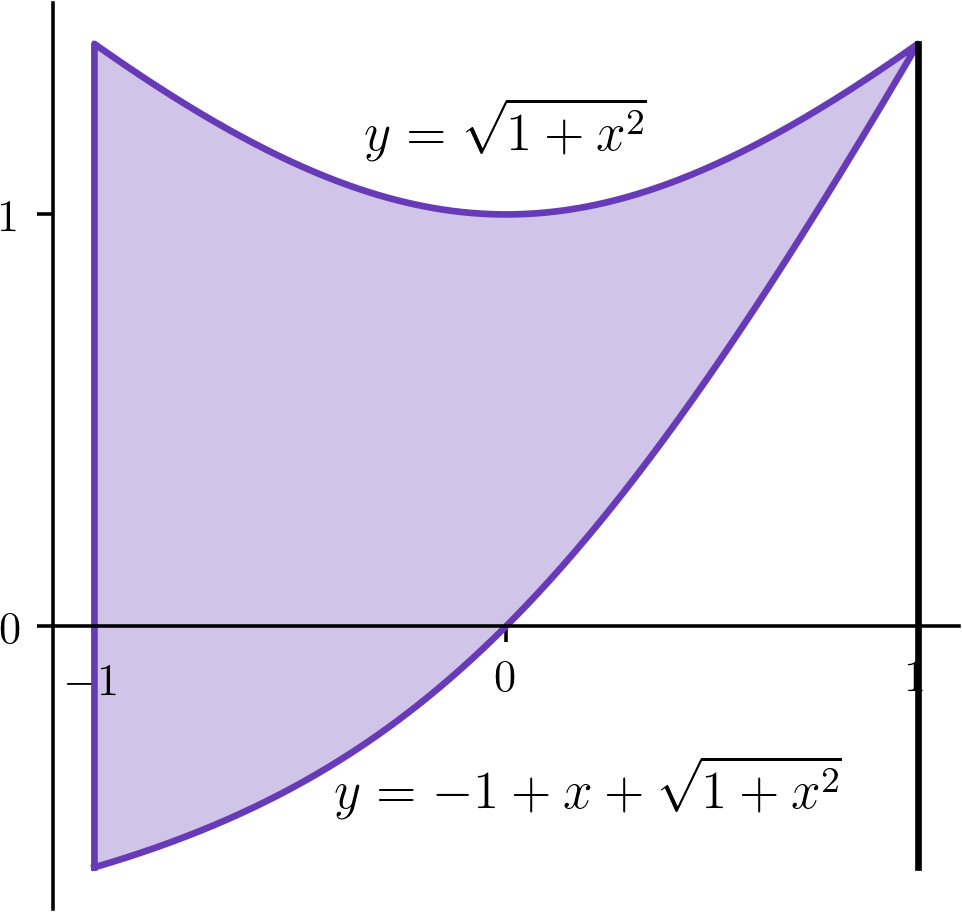
\includegraphics{shell/shell04.png}
\end{image}
\end{center}
\begin{itemize}
\item When the slicing variable is $x$, the radius of a shell is the \wordChoice{\choice[correct]{horizontal}\choice{vertical}} distance from an $x$-slice to the axis $x = 0$. Thus
\[ r(x) = \answer{1} - \answer{x}. \]
\item The height of an $x$-slice is equal to
\[ h(x) = \answer{-1+x}. \]
\item The volume is equal to the integral of $2 \pi r h$, so 
\[ V = \int_{\answer{-1}}^{\answer{1}} \answer{2 \pi (1-x)^2 } dx = \answer{\frac{16\pi}{3}}. \]
\end{itemize}
\end{exercise}


\section*{Sample Quiz Questions}

\begin{question}%%%%%[ShellQuad001]

The region in the plane bounded below by the curve \(y=-x^2\), above by the curve \(y=x^2+2x+2\), on the right by the line  \(x = 0\), and on the left by the line \(x = -2\) is revolved around the axis \(x = -2\). Compute the volume of the resulting solid.
\begin{multiplechoice}
\choice{\(4\pi\)}
\choice{\(6\pi\)}
\choice[correct]{\(8\pi\)}
\choice{\(10\pi\)}
\choice{\(12\pi\)}
\choice{\(14\pi\)}
\end{multiplechoice}
\begin{feedback}
The axis \(x = -2\) is parallel to the direction of slices using the integration variable \(x\), which indicates the shell method. 
 The region lies to the right of the axis, which must be the case because the interval \(-2 \leq x \leq 0\) lies to the right of the axis \(x = -2\).
The integral to compute equals \[ \begin{aligned} V &= \int_{-2}^{0}2 \pi (x-(-2))((x^2+2x+2)-(-x^2))~ dx\\
& = \pi \int_{-2}^{0} (4x^3+12x^2+12x+8)~ dx\\
& = \pi \left. \left(x^4+4x^3+6x^2+8x\right) \right|_{-2}^{0} = 8\pi. \end{aligned}\]
\end{feedback}

\end{question}

\begin{question}%%%%%[ShellQuad019]

The region in the plane bounded on the left by the curve \(x=-y^2+4y+1\), on the right by the curve \(x=y^2+2y+1\), and below by the line \(y = -1\) is revolved around the axis \(y = -1\). Compute the volume of the resulting solid.
\begin{multiplechoice}
\choice[correct]{\(\pi\)}
\choice{\(5\pi\)}
\choice{\(9\pi\)}
\choice{\(13\pi\)}
\choice{\(17\pi\)}
\choice{\(21\pi\)}
\end{multiplechoice}
\begin{feedback}
The axis \(y = -1\) is parallel to the direction of slices using the integration variable \(y\), which indicates the shell method. The lower endpoint of integration will be \(y = -1\); the upper endpoint can be determined by setting \(-y^2+4y+1 = y^2+2y+1\) and choosing the solution which is greater than \(-1\). This gives the range \(-1 \leq y \leq 0\). 
 The region lies above the axis, which must be the case because the interval \(-1 \leq y \leq 0\) lies above the axis \(y = -1\).
The integral to compute equals \[ \begin{aligned} V &= \int_{-1}^{0}2 \pi (y-(-1))((y^2+2y+1)-(-y^2+4y+1))~ dy\\
& = \pi \int_{-1}^{0} (4y^3-4y)~ dy\\
& = \pi \left. \left(y^4-2y^2\right) \right|_{-1}^{0} = 1\pi. \end{aligned}\]
\end{feedback}

\end{question}

\begin{question}%%%%%[shellalgsub2001]

The region in the plane between the  \(x\)-axis and the graph
\[ y = \frac{1}{2 \sqrt{\frac{x^{2}}{3} + 1}} \]
 in the range \(0 \leq x \leq 3\) is revolved around the axis \(x = 0\). Compute the volume of the resulting solid.
\begin{multiplechoice}
\choice{\(\displaystyle \frac{3}{2} \pi\)}
\choice{\(\displaystyle \frac{8}{5} \pi\)}
\choice{\(\displaystyle \frac{5}{3} \pi\)}
\choice{\(\displaystyle 2 \pi\)}
\choice[correct]{\(\displaystyle 3 \pi\)}
\choice{\(\displaystyle 5 \pi\)}
\end{multiplechoice}
\begin{feedback}
If the variable \(x\) is used for slicing, then slices are parallel to the axis of rotation, which indicates the shell method should be used.
The radius of a shell is \(x\). The height of a shell is exactly \(\frac{1}{2 \sqrt{\frac{x^{2}}{3} + 1}}\).
The volume of the region is therefore given by
\[ \int_{0}^{3} \frac{\sqrt{3} \pi x}{\sqrt{x^{2} + 3}}\, dx. \]
 To compute the integral we can use the substitution \(u = x^{2} + 3\) which implies the equality \(du = \left(2 x\right)dx\) for the differentials. This gives the equality
\[ \begin{aligned} \int \frac{\sqrt{3} \pi x}{\sqrt{x^{2} + 3}}\, dx & = \int \frac{\sqrt{3} \pi}{2 \sqrt{u}}\, du \\
 & = \sqrt{3} \pi \sqrt{u}. \end{aligned} \]
Reversing the substitution gives
\[ \begin{aligned} \int_{0}^{3} \frac{\sqrt{3} \pi x}{\sqrt{x^{2} + 3}}\, dx & = \left. \left[\sqrt{3} \pi \sqrt{x^{2} + 3} \right] \right|_{0}^{3}\\ & = \left(6 \pi \right) - \left(3 \pi \right) = 3 \pi. \end{aligned} \]
\end{feedback}

\end{question}





\end{document}
